

We include auxiliary plots for the Couplings Analysis.

%\begin{center}
%        \foreach \i in {2,...,89}{%
%                \includegraphics[width=0.3\linewidth]{figures/couplings_chapter/plot_singleRes_m125_c\i}
%        }
%        \begin{figure}[h]
%                \caption{Fitted Double Sided Crystal ball shapes for all 88 analysis categories.}
%                \label{fig:signal_shapes}
%        \end{figure}
%\end{center}

\begin{landscape}
\begin{figure}[h]
\centering
\includegraphics[width=1.5\textwidth]{figures/couplings_chapter/purity_2D.pdf}
\caption{Contribution of STXS truth bins to each analysis category in total event yield. The top row corresponds to the value of $S_{90}/(S_{90} + B_{90})$ in each category, where $S_{90}$ and $B_{90}$ are respectively the total number of signal (including all STXS regions) and background events expected in the smallest $m_{\gamma \gamma}$ range containing 90\% of the signal yield. Other entries correspond to the percentage contribution of a given STXS truth bin to the Higgs signal yield in each analysis category. Entries for the STXS regions targeted by each analysis category are outlined in black if this value is above 15\%. }
\label{fig:design:yields}
\end{figure}
\end{landscape}

\begin{figure}[htbp]
  \centering
  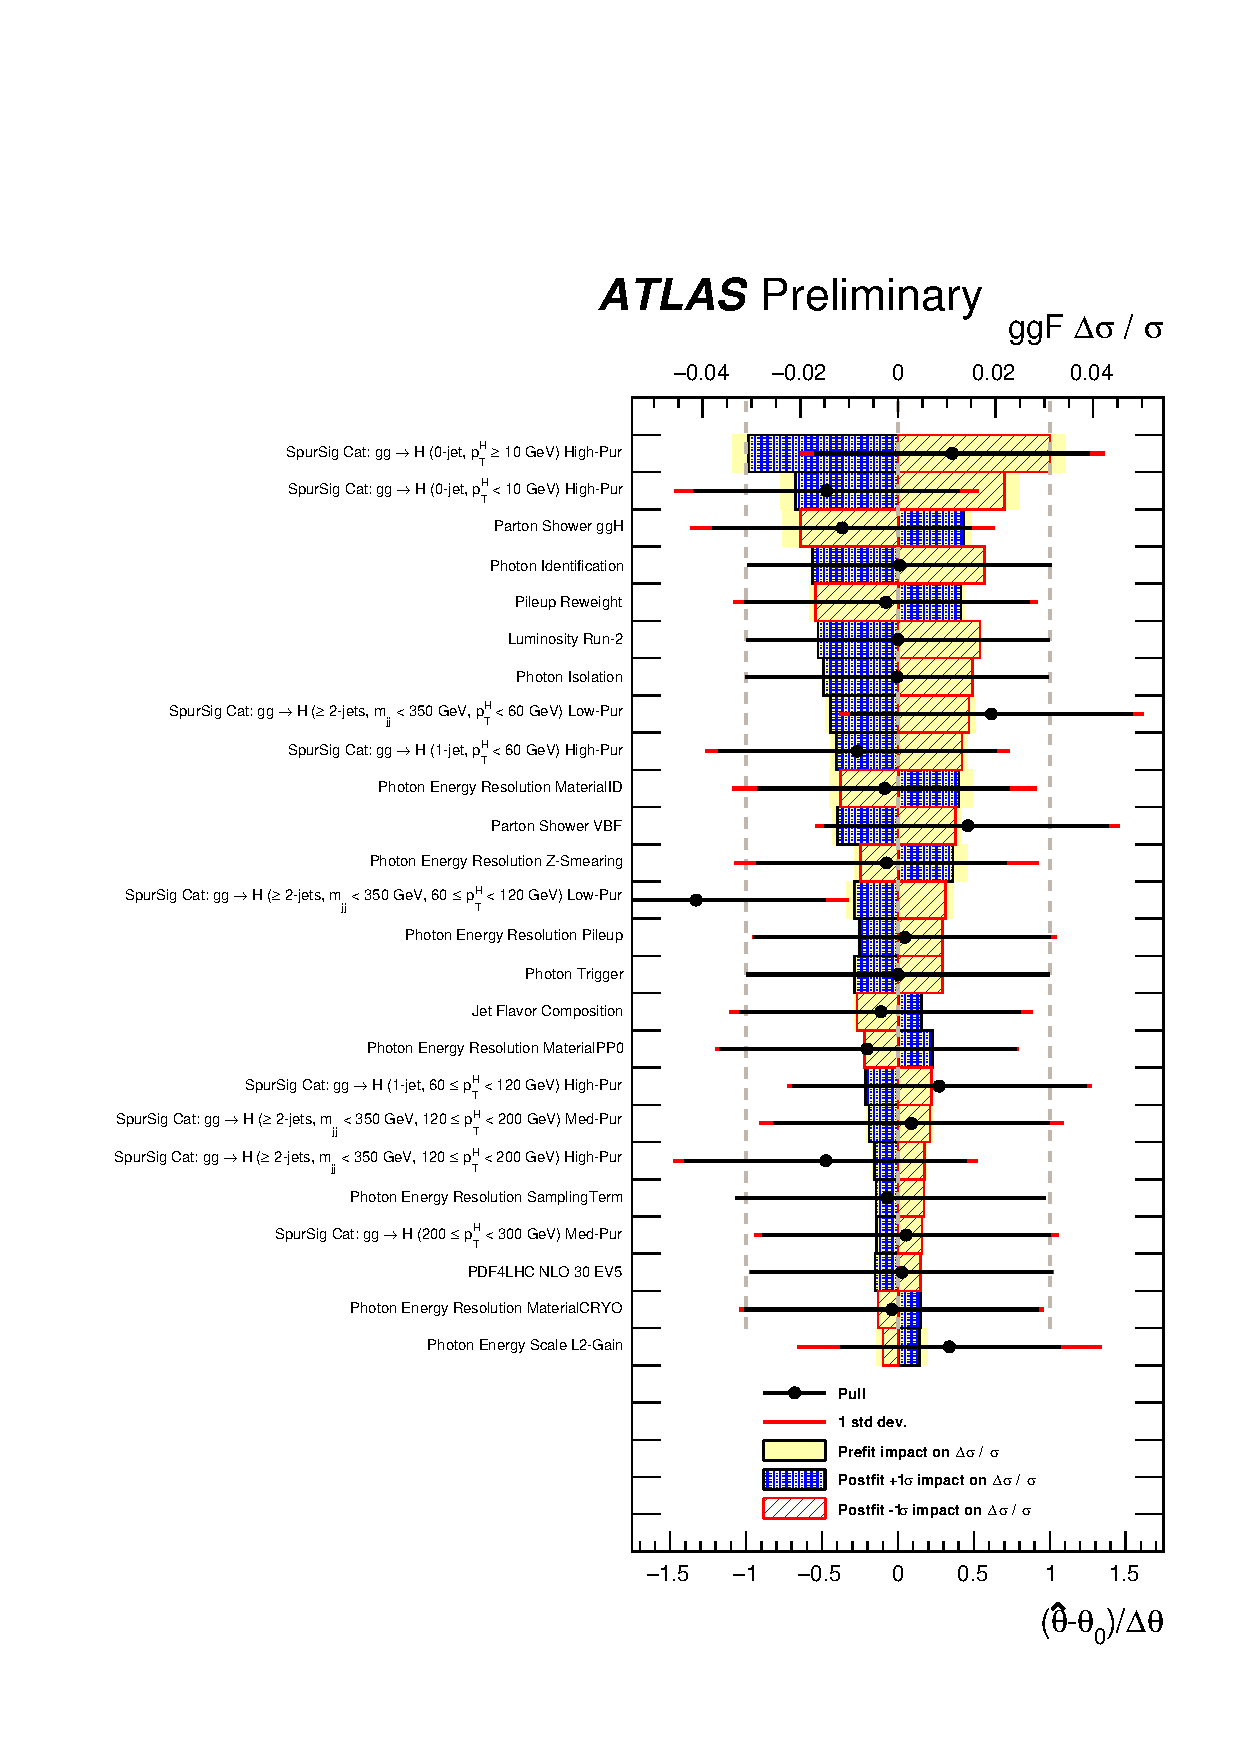
\includegraphics[width=0.9\linewidth]{figures/couplings_chapter/pulls_mu_ggF}
  \caption{Nuisance parameter "pull plots" for the $ggH$ cross-section in the five-production-mode fit. The nuisance parameters are ranked by their impact on the cross-section measurement. These show the pre-fit and post-fit impact of various nuisance parameters on the cross-section measurement (colored and shaded boxes, corresponding to the top x-axis), as well as the "pull" (change in mean and spread between pre- and post-fit nuisance parameters, corresponding to the bottom x-axis).}
  \label{fig:ranking_ggF}
\end{figure}

\begin{figure}[htbp]
  \centering
  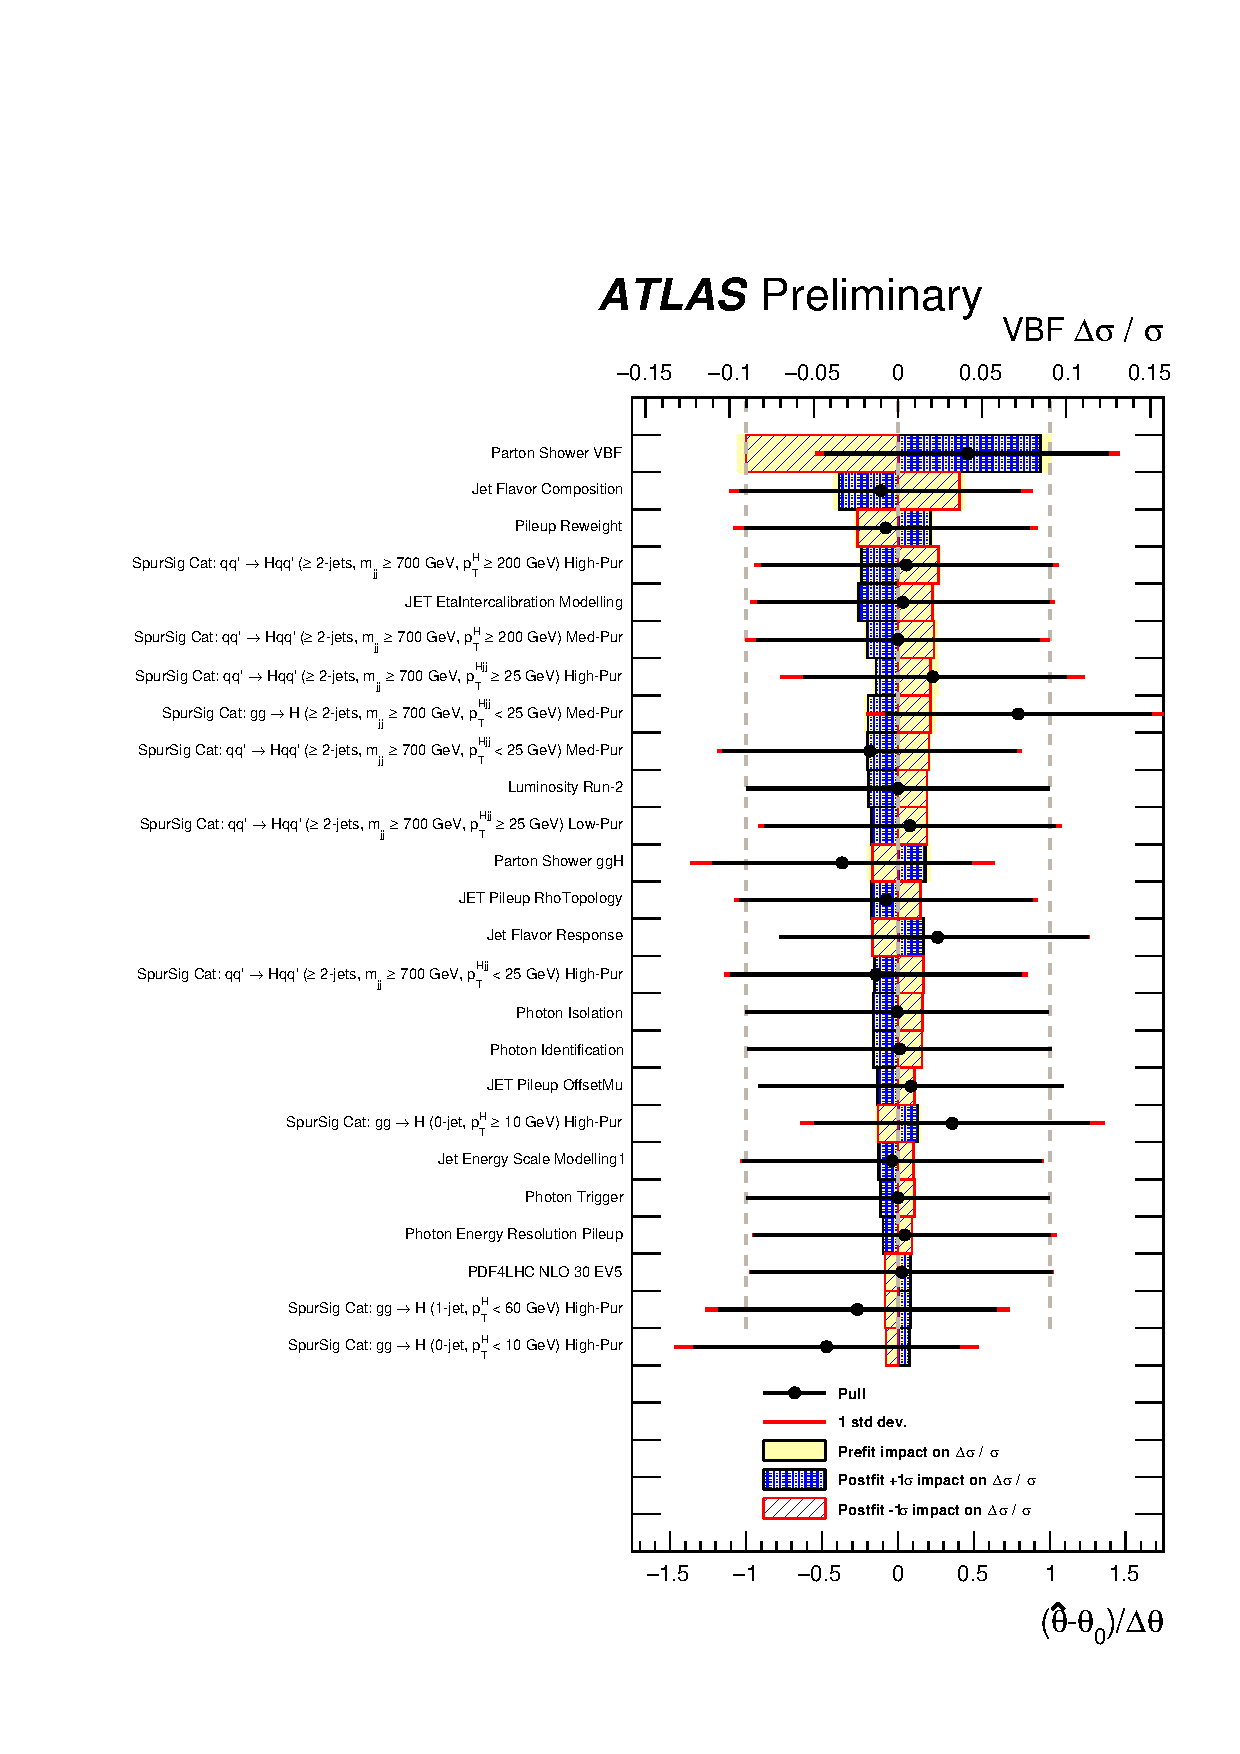
\includegraphics[width=0.9\linewidth]{figures/couplings_chapter/pulls_mu_VBF}
  \caption{Nuisance parameter "pull plots" for the $VBF$ cross-section in the five-production-mode fit. The nuisance parameters are ranked by their impact on the cross-section measurement. These show the pre-fit and post-fit impact of various nuisance parameters on the cross-section measurement (colored and shaded boxes, corresponding to the top x-axis), as well as the "pull" (change in mean and spread between pre- and post-fit nuisance parameters, corresponding to the bottom x-axis).}
  \label{fig:ranking_VBF}
\end{figure}

\begin{figure}[htbp]
  \centering
  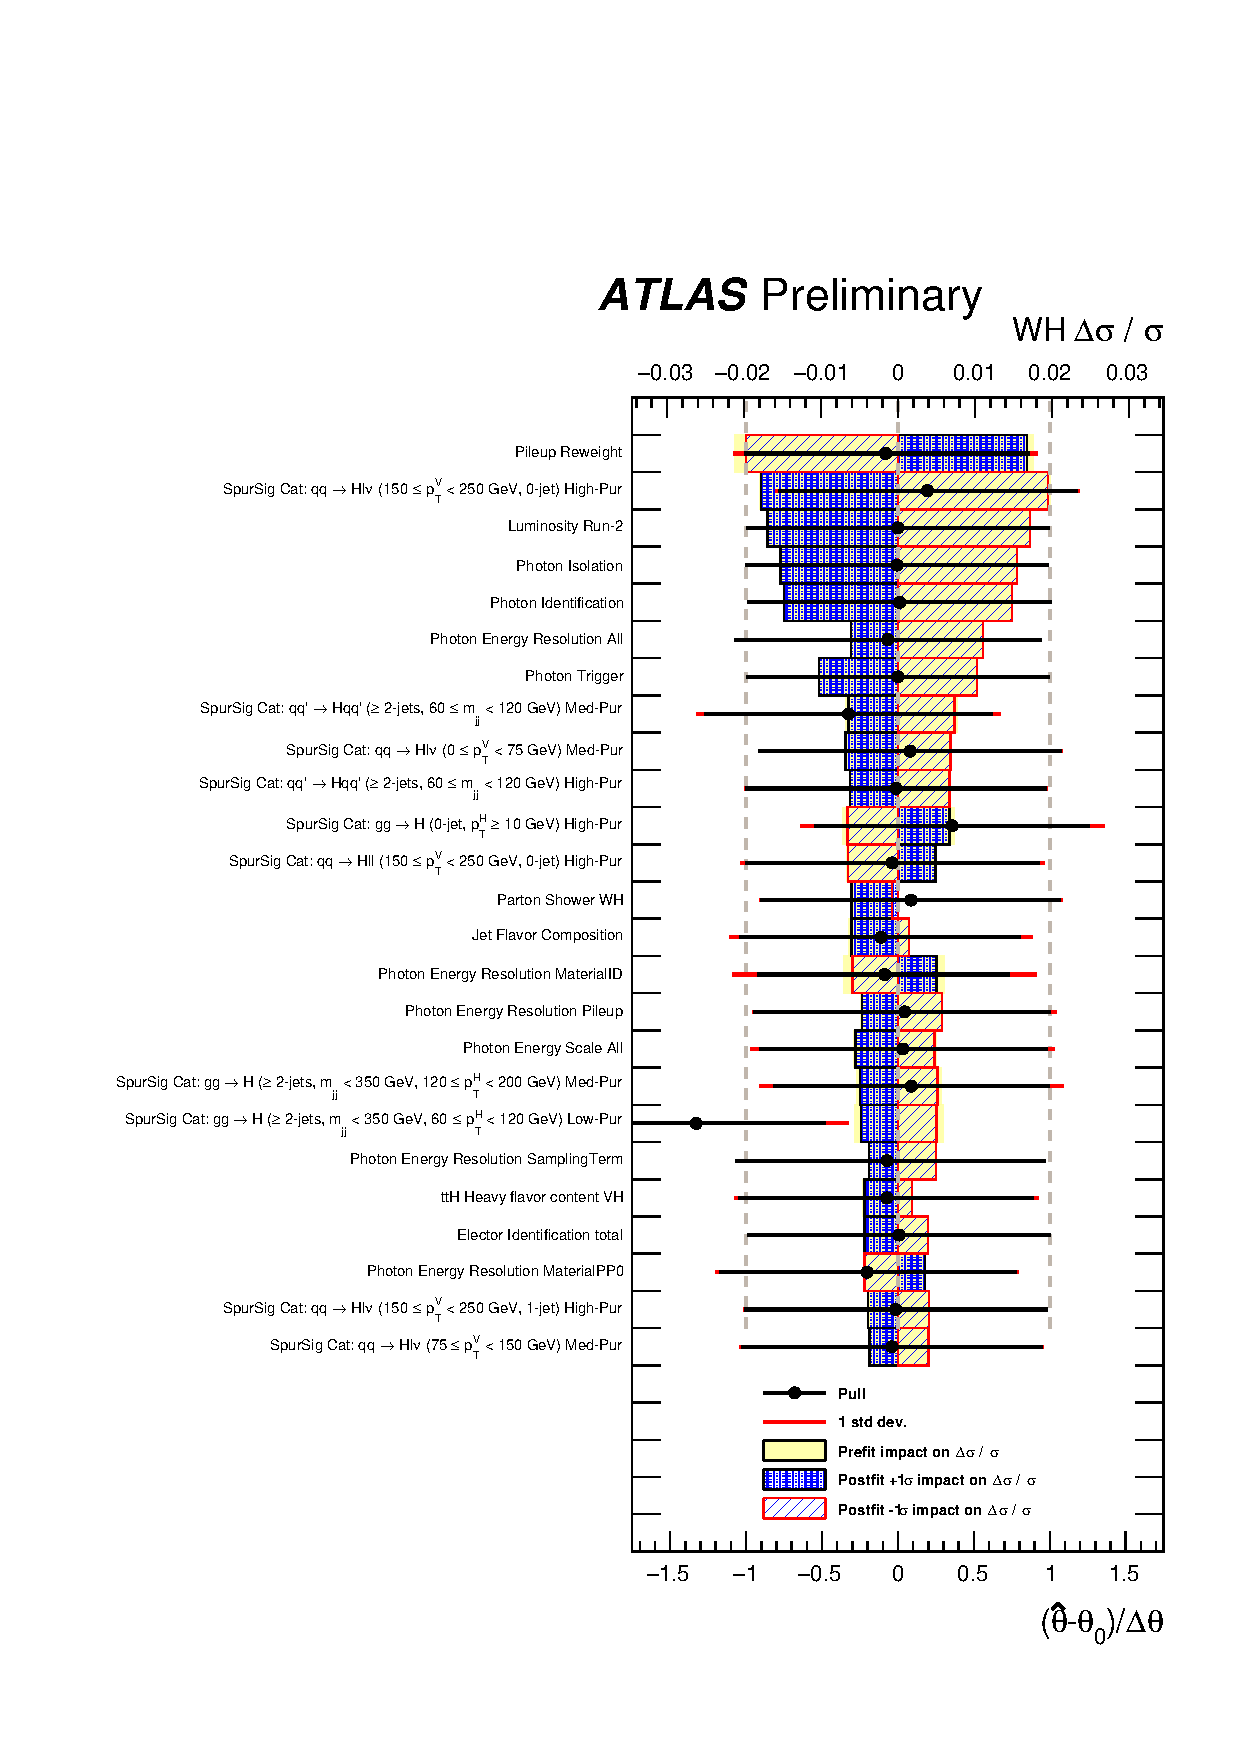
\includegraphics[width=0.9\linewidth]{figures/couplings_chapter/pulls_mu_WH}
  \caption{Nuisance parameter "pull plots" for the $WH$ cross-section in the five-production-mode fit. The nuisance parameters are ranked by their impact on the cross-section measurement. These show the pre-fit and post-fit impact of various nuisance parameters on the cross-section measurement (colored and shaded boxes, corresponding to the top x-axis), as well as the "pull" (change in mean and spread between pre- and post-fit nuisance parameters, corresponding to the bottom x-axis).}
  \label{fig:ranking_WH}
\end{figure}

\begin{figure}[htbp]
  \centering
  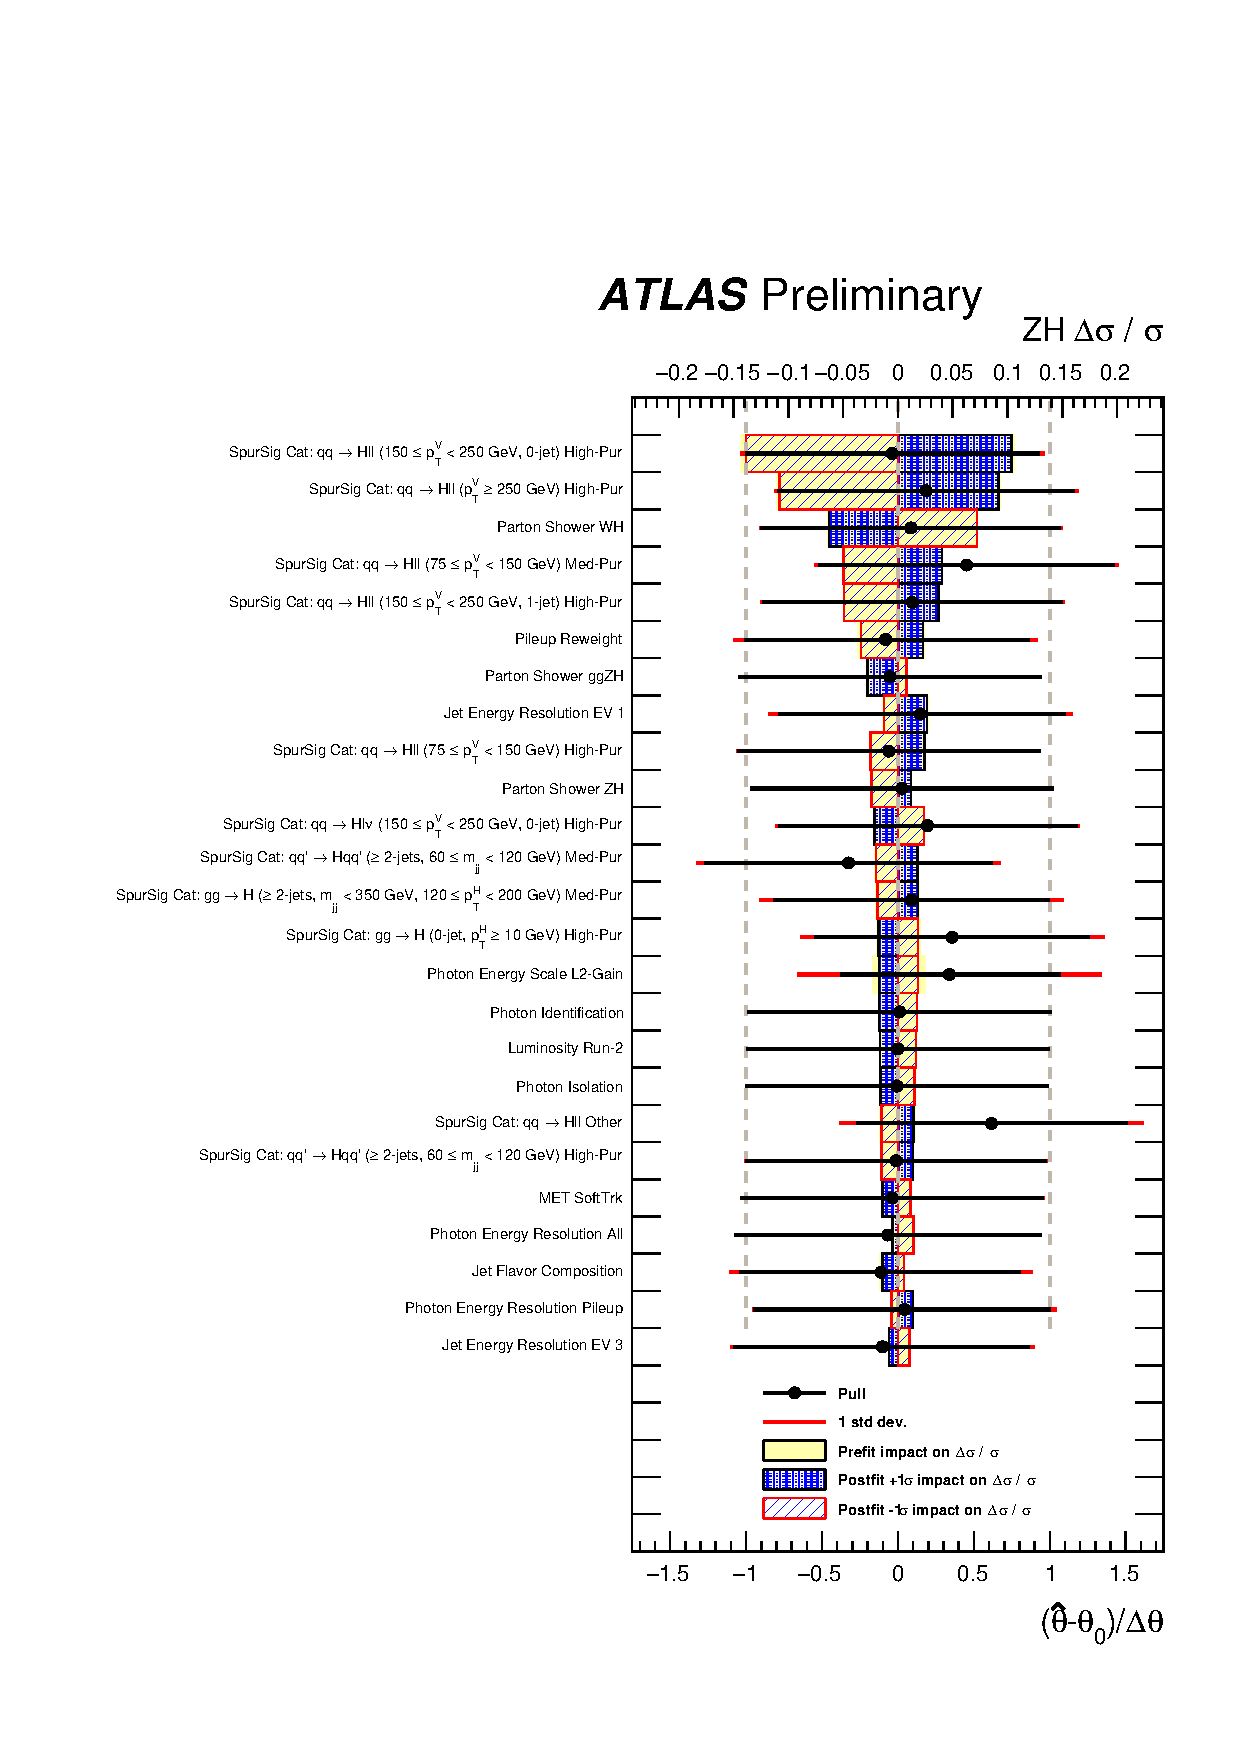
\includegraphics[width=0.9\linewidth]{figures/couplings_chapter/pulls_mu_ZH}
  \caption{Nuisance parameter "pull plots" for the $ZH$ cross-section in the five-production-mode fit. The nuisance parameters are ranked by their impact on the cross-section measurement. These show the pre-fit and post-fit impact of various nuisance parameters on the cross-section measurement (colored and shaded boxes, corresponding to the top x-axis), as well as the "pull" (change in mean and spread between pre- and post-fit nuisance parameters, corresponding to the bottom x-axis).}
  \label{fig:ranking_ZH}
\end{figure}

\begin{figure}[htbp]
  \centering
  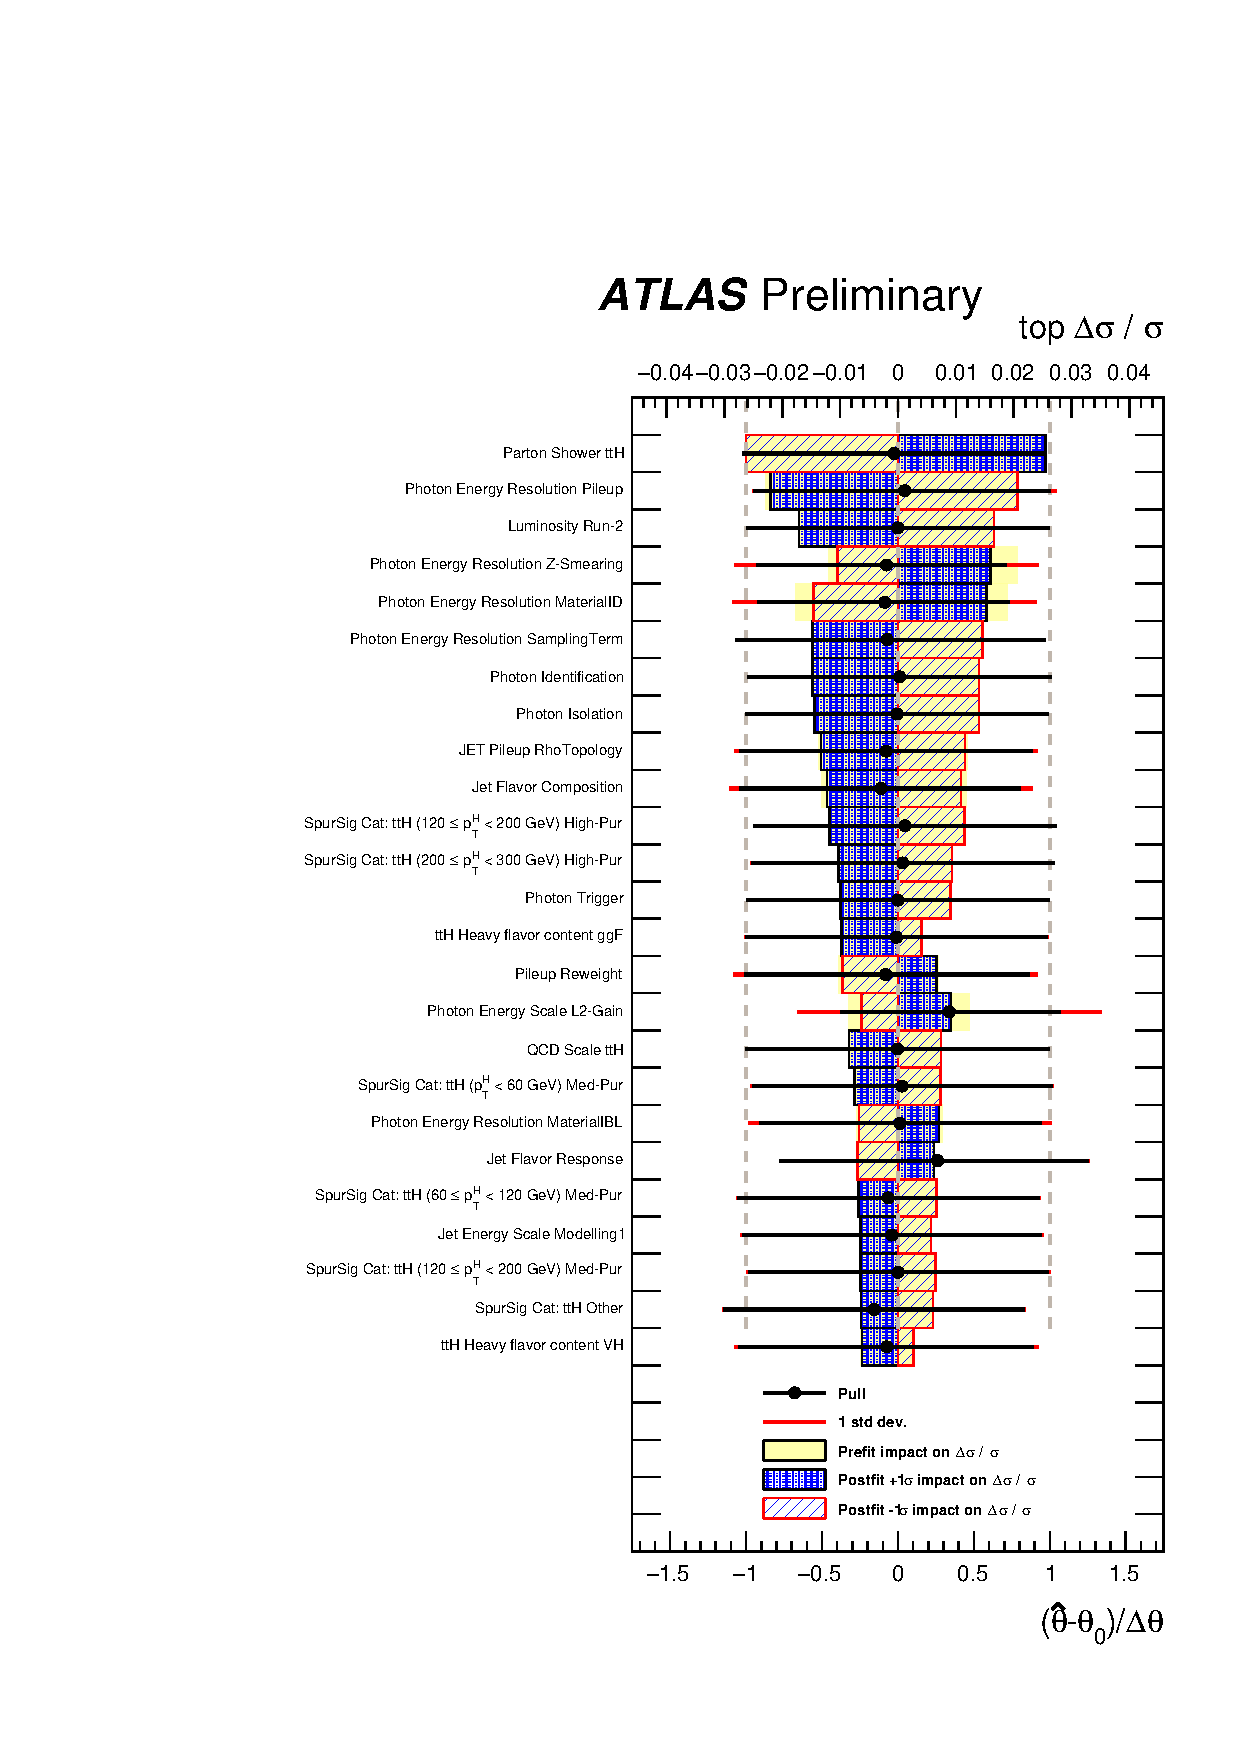
\includegraphics[width=0.9\linewidth]{figures/couplings_chapter/pulls_mu_top}
  \caption{Nuisance parameter "pull plots" for the $ttH$+$tH$ cross-section in the five-production-mode fit. The nuisance parameters are ranked by their impact on the cross-section measurement. These show the pre-fit and post-fit impact of various nuisance parameters on the cross-section measurement (colored and shaded boxes, corresponding to the top x-axis), as well as the "pull" (change in mean and spread between pre- and post-fit nuisance parameters, corresponding to the bottom x-axis).}
  \label{fig:ranking_top}
\end{figure}
